\chapter{Managing change with Mercurial Queues}
\label{chap:mq}

\section{The patch management problem}
\label{sec:mq:patch-mgmt}

Here is a common scenario: you need to install a software package from
source, but you find a bug that you must fix in the source before you
can start using the package.  You make your changes, forget about the
package for a while, and a few months later you need to upgrade to a
newer version of the package.  If the newer version of the package
still has the bug, you must extract your fix from the older source
tree and apply it against the newer version.  This is a tedious task,
and it's easy to make mistakes.

This is a simple case of the ``patch management'' problem.  You have
an ``upstream'' source tree that you can't change; you need to make
some local changes on top of the upstream tree; and you'd like to be
able to keep those changes separate, so that you can apply them to
newer versions of the upstream source.

The patch management problem arises in many situations.  Probably the
most visible is that a user of an open source software project will
contribute a bug fix or new feature to the project's maintainers in the
form of a patch.

Distributors of operating systems that include open source software
often need to make changes to the packages they distribute so that
they will build properly in their environments.

When you have few changes to maintain, it is easy to manage a single
patch using the standard \texttt{diff} and \texttt{patch} programs
(see section~\ref{sec:mq:patch} for a discussion of these tools).
Once the number of changes grows, it starts to makes sense to maintain
patches as discrete ``chunks of work,'' so that for example a single
patch will contain only one bug fix (the patch might modify several
files, but it's doing ``only one thing''), and you may have a number
of such patches for different bugs you need fixed and local changes
you require.  In this situation, if you submit a bug fix patch to the
upstream maintainers of a package and they include your fix in a
subsequent release, you can simply drop that single patch when you're
updating to the newer release.

Maintaining a single patch against an upstream tree is a little
tedious and error-prone, but not difficult.  However, the complexity
of the problem grows rapidly as the number of patches you have to
maintain increases.  With more than a tiny number of patches in hand,
understanding which ones you have applied and maintaining them moves
from messy to overwhelming.

Fortunately, Mercurial includes a powerful extension, Mercurial Queues
(or simply ``MQ''), that massively simplifies the patch management
problem.

\section{The prehistory of Mercurial Queues}
\label{sec:mq:history}

During the late 1990s, several Linux kernel developers started to
maintain ``patch series'' that modified the behaviour of the Linux
kernel.  Some of these series were focused on stability, some on
feature coverage, and others were more speculative.

The sizes of these patch series grew rapidly.  In 2002, Andrew Morton
published some shell scripts he had been using to automate the task of
managing his patch queues.  Andrew was successfully using these
scripts to manage hundreds (sometimes thousands) of patches on top of
the Linux kernel.

\subsection{A patchwork quilt}
\label{sec:mq:quilt}


In early 2003, Andreas Gruenbacher and Martin Quinson borrowed the
approach of Andrew's scripts and published a tool called ``patchwork
quilt''~\cite{web:quilt}, or simply ``quilt''
(see~\cite{gruenbacher:2005} for a paper describing it).  Because
quilt substantially automated patch management, it rapidly gained a
large following among open source software developers.

Quilt manages a \emph{stack of patches} on top of a directory tree.
To begin, you tell quilt to manage a directory tree, and tell it which
files you want to manage; it stores away the names and contents of
those files.  To fix a bug, you create a new patch (using a single
command), edit the files you need to fix, then ``refresh'' the patch.

The refresh step causes quilt to scan the directory tree; it updates
the patch with all of the changes you have made.  You can create
another patch on top of the first, which will track the changes
required to modify the tree from ``tree with one patch applied'' to
``tree with two patches applied''.

You can \emph{change} which patches are applied to the tree.  If you
``pop'' a patch, the changes made by that patch will vanish from the
directory tree.  Quilt remembers which patches you have popped,
though, so you can ``push'' a popped patch again, and the directory
tree will be restored to contain the modifications in the patch.  Most
importantly, you can run the ``refresh'' command at any time, and the
topmost applied patch will be updated.  This means that you can, at
any time, change both which patches are applied and what
modifications those patches make.

Quilt knows nothing about revision control tools, so it works equally
well on top of an unpacked tarball or a Subversion repository.

\subsection{From patchwork quilt to Mercurial Queues}
\label{sec:mq:quilt-mq}

In mid-2005, Chris Mason took the features of quilt and wrote an
extension that he called Mercurial Queues, which added quilt-like
behaviour to Mercurial.

The key difference between quilt and MQ is that quilt knows nothing
about revision control systems, while MQ is \emph{integrated} into
Mercurial.  Each patch that you push is represented as a Mercurial
changeset.  Pop a patch, and the changeset goes away.

This integration makes understanding patches and debugging their
effects \emph{enormously} easier.  Since every applied patch has an
associated changeset, you can use \hgcmdargs{log}{\emph{filename}} to
see which changesets and patches affected a file.  You can use the
\hgext{bisect} extension to binary-search through all changesets and
applied patches to see where a bug got introduced or fixed.  You can
use the \hgcmd{annotate} command to see which changeset or patch
modified a particular line of a source file.  And so on.

Because quilt does not care about revision control tools, it is still
a tremendously useful piece of software to know about for situations
where you cannot use Mercurial and MQ.

\section{Understanding patches}
\label{sec:mq:patch}

Because MQ doesn't hide its patch-oriented nature, it is helpful to
understand what patches are, and a little about the tools that work
with them.

The traditional Unix \command{diff} command compares two files, and
prints a list of differences between them. The \command{patch} command
understands these differences as \emph{modifications} to make to a
file.  Take a look at figure~\ref{ex:mq:diff} for a simple example of
these commands in action.

\begin{figure}[ht]
  \interaction{mq.diff.diff}
  \caption{Simple uses of the \command{diff} and \command{patch} commands}
  \label{ex:mq:diff}
\end{figure}

The type of file that \command{diff} generates (and \command{patch}
takes as input) is called a ``patch'' or a ``diff''; there is no
difference between a patch and a diff.  (We'll use the term ``patch'',
since it's more commonly used.)

A patch file can start with arbitrary text; the \command{patch}
command ignores this text, but MQ uses it as the commit message when
creating changesets.  To find the beginning of the patch content,
\command{patch} searches for the first line that starts with the
string ``\texttt{diff~-}''.

MQ works with \emph{unified} diffs (\command{patch} can accept several
other diff formats, but MQ doesn't).  A unified diff contains two
kinds of header.  The \emph{file header} describes the file being
modified; it contains the name of the file to modify.  When
\command{patch} sees a new file header, it looks for a file with that
name to start modifying.

After the file header comes a series of \emph{hunks}.  Each hunk
starts with a header; this identifies the range of line numbers within
the file that the hunk should modify.  Following the header, a hunk
starts and ends with a few (usually three) lines of text from the
unmodified file; these are called the \emph{context} for the hunk.  If
there's only a small amount of context between successive hunks,
\command{diff} doesn't print a new hunk header; it just runs the hunks
together, with a few lines of context between modifications.

Each line of context begins with a space character.  Within the hunk,
a line that begins with ``\texttt{-}'' means ``remove this line,''
while a line that begins with ``\texttt{+}'' means ``insert this
line.''  For example, a line that is modified is represented by one
deletion and one insertion.

We will return to ome of the more subtle aspects of patches later (in
section~\ref{sec:mq:adv-patch}), but you should have enough information
now to use MQ.

\section{Getting started with Mercurial Queues}
\label{sec:mq:start}

Because MQ is implemented as an extension, you must explicitly enable
before you can use it.  (You don't need to download anything; MQ ships
with the standard Mercurial distribution.)  To enable MQ, edit your
\tildefile{.hgrc} file, and add the lines in figure~\ref{ex:mq:config}.

\begin{figure}[ht]
  \begin{codesample4}
    [extensions]
    hgext.mq =
  \end{codesample4}
  \label{ex:mq:config}
  \caption{Contents to add to \tildefile{.hgrc} to enable the MQ extension}
\end{figure}

Once the extension is enabled, it will make a number of new commands
available.  To verify that the extension is working, you can use
\hgcmd{help} to see if the \hgcmd{qinit} command is now available; see
the example in figure~\ref{ex:mq:enabled}.

\begin{figure}[ht]
  \interaction{mq.qinit-help.help}
  \caption{How to verify that MQ is enabled}
  \label{ex:mq:enabled}
\end{figure}

You can use MQ with \emph{any} Mercurial repository, and its commands
only operate within that repository.  To get started, simply prepare
the repository using the \hgcmd{qinit} command (see
figure~\ref{ex:mq:qinit}).  This command creates an empty directory
called \sdirname{.hg/patches}, where MQ will keep its metadata.  As
with many Mercurial commands, the \hgcmd{qinit} command prints nothing
if it succeeds.

\begin{figure}[ht]
  \interaction{mq.tutorial.qinit}
  \caption{Preparing a repository for use with MQ}
  \label{ex:mq:qinit}
\end{figure}

\begin{figure}[ht]
  \interaction{mq.tutorial.qnew}
  \caption{Creating a new patch}
  \label{ex:mq:qnew}
\end{figure}

\subsection{Creating a new patch}

To begin work on a new patch, use the \hgcmd{qnew} command.  This
command takes one argument, the name of the patch to create.  MQ will
use this as the name of an actual file in the \sdirname{.hg/patches}
directory, as you can see in figure~\ref{ex:mq:qnew}.

Also newly present in the \sdirname{.hg/patches} directory are two
other files, \sfilename{series} and \sfilename{status}.  The
\sfilename{series} file lists all of the patches that MQ knows about
for this repository, with one patch per line.  Mercurial uses the
\sfilename{status} file for internal book-keeping; it tracks all of the
patches that MQ has \emph{applied} in this repository.

\begin{note}
  You may sometimes want to edit the \sfilename{series} file by hand;
  for example, to change the sequence in which some patches are
  applied.  However, manually editing the \sfilename{status} file is
  almost always a bad idea, as it's easy to corrupt MQ's idea of what
  is happening.
\end{note}

Once you have created your new patch, you can edit files in the
working directory as you usually would.  All of the normal Mercurial
commands, such as \hgcmd{diff} and \hgcmd{annotate}, work exactly as
they did before.

\subsection{Refreshing a patch}

When you reach a point where you want to save your work, use the
\hgcmd{qrefresh} command (figure~\ref{ex:mq:qnew}) to update the patch
you are working on.  This command folds the changes you have made in
the working directory into your patch, and updates its corresponding
changeset to contain those changes.

\begin{figure}[ht]
  \interaction{mq.tutorial.qrefresh}
  \caption{Refreshing a patch}
  \label{ex:mq:qrefresh}
\end{figure}

You can run \hgcmd{qrefresh} as often as you like, so it's a good way
to ``checkpoint'' your work.  Refresh your patch at an opportune
time; try an experiment; and if the experiment doesn't work out,
\hgcmd{revert} your modifications back to the last time you refreshed.

\begin{figure}[ht]
  \interaction{mq.tutorial.qrefresh2}
  \caption{Refresh a patch many times to accumulate changes}
  \label{ex:mq:qrefresh2}
\end{figure}

\subsection{Stacking and tracking patches}

Once you have finished working on a patch, or need to work on another,
you can use the \hgcmd{qnew} command again to create a new patch.
Mercurial will apply this patch on top of your existing patch.  See
figure~\ref{ex:mq:qnew2} for an example.  Notice that the patch
contains the changes in our prior patch as part of its context (you
can see this more clearly in the output of \hgcmd{annotate}).

\begin{figure}[ht]
  \interaction{mq.tutorial.qnew2}
  \caption{Stacking a second patch on top of the first}
  \label{ex:mq:qnew2}
\end{figure}

So far, with the exception of \hgcmd{qnew} and \hgcmd{qrefresh}, we've
been careful to only use regular Mercurial commands.  However, MQ
provides many commands that are easier to use when you are thinking
about patches, as illustrated in figure~\ref{ex:mq:qseries}:

\begin{itemize}
\item The \hgcmd{qseries} command lists every patch that MQ knows
  about in this repository, from oldest to newest (most recently
  \emph{created}).
\item The \hgcmd{qapplied} command lists every patch that MQ has
  \emph{applied} in this repository, again from oldest to newest (most
  recently applied).
\end{itemize}

\begin{figure}[ht]
  \interaction{mq.tutorial.qseries}
  \caption{Understanding the patch stack with \hgcmd{qseries} and
    \hgcmd{qapplied}}
  \label{ex:mq:qseries}
\end{figure}

\subsection{Manipulating the patch stack}

The previous discussion implied that there must be a difference
between ``known'' and ``applied'' patches, and there is.  MQ can
manage a patch without it being applied in the repository.

An \emph{applied} patch has a corresponding changeset in the
repository, and the effects of the patch and changeset are visible in
the working directory.  You can undo the application of a patch using
the \hgcmd{qpop} command.  MQ still \emph{knows about}, or manages, a
popped patch, but the patch no longer has a corresponding changeset in
the repository, and the working directory does not contain the changes
made by the patch.  Figure~\ref{fig:mq:stack} illustrates the
difference between applied and tracked patches.

\begin{figure}[ht]
  \centering
  \includegraphics{mq-stack}
  \caption{Applied and unapplied patches in the MQ patch stack}
  \label{fig:mq:stack}
\end{figure}

You can reapply an unapplied, or popped, patch using the \hgcmd{qpush}
command.  This creates a new changeset to correspond to the patch, and
the patch's changes once again become present in the working
directory.  See figure~\ref{ex:mq:qpop} for examples of \hgcmd{qpop}
and \hgcmd{qpush} in action.  Notice that once we have popped a patch
or two patches, the output of \hgcmd{qseries} remains the same, while
that of \hgcmd{qapplied} has changed.

\begin{figure}[ht]
  \interaction{mq.tutorial.qpop}
  \caption{Modifying the stack of applied patches}
  \label{ex:mq:qpop}
\end{figure}

\subsection{Pushing and popping many patches}

While \hgcmd{qpush} and \hgcmd{qpop} each operate on a single patch at
a time by default, you can push and pop many patches in one go.  The
\hgopt{qpush}{-a} option to \hgcmd{qpush} causes it to push all
unapplied patches, while the \hgopt{qpop}{-a} option to \hgcmd{qpop}
causes it to pop all applied patches.  (For some more ways to push and
pop many patches, see section~\ref{sec:mq:perf} below.)

\begin{figure}[ht]
  \interaction{mq.tutorial.qpush-a}
  \caption{Pushing all unapplied patches}
  \label{ex:mq:qpush-a}
\end{figure}

\subsection{Safety checks, and overriding them}

Several MQ commands check the working directory before they do
anything, and fail if they find any modifications.  They do this to
ensure that you won't lose any changes that you have made, but not yet
incorporated into a patch.  Figure~\ref{ex:mq:add} illustrates this;
the \hgcmd{qnew} command will not create a new patch if there are
outstanding changes, caused in this case by the \hgcmd{add} of
\filename{file3}.

\begin{figure}[ht]
  \interaction{mq.tutorial.add}
  \caption{Forcibly creating a patch}
  \label{ex:mq:add}
\end{figure}

Commands that check the working directory all take an ``I know what
I'm doing'' option, which is always named \option{-f}.  The exact
meaning of \option{-f} depends on the command.  For example,
\hgcmdargs{qnew}{\hgopt{qnew}{-f}} will incorporate any outstanding
changes into the new patch it creates, but
\hgcmdargs{qpop}{\hgopt{qpop}{-f}} will revert modifications to any
files affected by the patch that it is popping.  Be sure to read the
documentation for a command's \option{-f} option before you use it!

\subsection{Working on several patches at once}

The \hgcmd{qrefresh} command always refreshes the \emph{topmost}
applied patch.  This means that you can suspend work on one patch (by
refreshing it), pop or push to make a different patch the top, and
work on \emph{that} patch for a while.

Here's an example that illustrates how you can use this ability.
Let's say you're developing a new feature as two patches.  The first
is a change to the core of your software, and the second---layered on
top of the first---changes the user interface to use the code you just
added to the core.  If you notice a bug in the core while you're
working on the UI patch, it's easy to fix the core.  Simply
\hgcmd{qrefresh} the UI patch to save your in-progress changes, and
\hgcmd{qpop} down to the core patch.  Fix the core bug,
\hgcmd{qrefresh} the core patch, and \hgcmd{qpush} back to the UI
patch to continue where you left off.

\section{More about patches}
\label{sec:mq:adv-patch}

MQ uses the GNU \command{patch} command to apply patches, so it's
helpful to know a few more detailed aspects of how \command{patch}
works, and about patches themselves.

\subsection{The strip count}

If you look at the file headers in a patch, you will notice that the
pathnames usually have an extra component on the front that isn't
present in the actual path name.  This is a holdover from the way that
people used to generate patches (people still do this, but it's
somewhat rare with modern revision control tools).  

Alice would unpack a tarball, edit her files, then decide that she
wanted to create a patch.  So she'd rename her working directory,
unpack the tarball again (hence the need for the rename), and use the
\cmdopt{diff}{-r} and \cmdopt{diff}{-N} options to \command{diff} to
recursively generate a patch between the unmodified directory and the
modified one.  The result would be that the name of the unmodified
directory would be at the front of the left-hand path in every file
header, and the name of the modified directory would be at the front
of the right-hand path.

Since someone receiving a patch from the Alices of the net would be
unlikely to have unmodified and modified directories with exactly the
same names, the \command{patch} command has a \cmdopt{patch}{-p}
option that indicates the number of leading path name components to
strip when trying to apply a patch.  This number is called the
\emph{strip count}.

An option of ``\texttt{-p1}'' means ``use a strip count of one''.  If
\command{patch} sees a file name \filename{foo/bar/baz} in a file
header, it will strip \filename{foo} and try to patch a file named
\filename{bar/baz}.  (Strictly speaking, the strip count refers to the
number of \emph{path separators} (and the components that go with them
) to strip.  A strip count of one will turn \filename{foo/bar} into
\filename{bar}, but \filename{/foo/bar} (notice the extra leading
slash) into \filename{foo/bar}.)

The ``standard'' strip count for patches is one; almost all patches
contain one leading path name component that needs to be stripped.
Mercurial's \hgcmd{diff} command generates path names in this form,
and the \hgcmd{import} command and MQ expect patches to have a strip
count of one.

If you receive a patch from someone that you want to add to your patch
queue, and the patch needs a strip count other than one, you cannot
just \hgcmd{qimport} the patch, because \hgcmd{qimport} does not yet
have a \texttt{-p} option (see~\bug{311}).  Your best bet is to
\hgcmd{qnew} a patch of your own, then use \cmdargs{patch}{-p\emph{N}}
to apply their patch, followed by \hgcmd{addremove} to pick up any
files added or removed by the patch, followed by \hgcmd{qrefresh}.
This complexity may become unnecessary; see~\bug{311} for details.
\subsection{Strategies for applying a patch}

When \command{patch} applies a hunk, it tries a handful of
successively less accurate strategies to try to make the hunk apply.
This falling-back technique often makes it possible to take a patch
that was generated against an old version of a file, and apply it
against a newer version of that file.

First, \command{patch} tries an exact match, where the line numbers,
the context, and the text to be modified must apply exactly.  If it
cannot make an exact match, it tries to find an exact match for the
context, without honouring the line numbering information.  If this
succeeds, it prints a line of output saying that the hunk was applied,
but at some \emph{offset} from the original line number.

If a context-only match fails, \command{patch} removes the first and
last lines of the context, and tries a \emph{reduced} context-only
match.  If the hunk with reduced context succeeds, it prints a message
saying that it applied the hunk with a \emph{fuzz factor} (the number
after the fuzz factor indicates how many lines of context
\command{patch} had to trim before the patch applied).

When neither of these techniques works, \command{patch} prints a
message saying that the hunk in question was rejected.  It saves
rejected hunks (also simply called ``rejects'') to a file with the
same name, and an added \sfilename{.rej} extension.  It also saves an
unmodified copy of the file with a \sfilename{.orig} extension; the
copy of the file without any extensions will contain any changes made
by hunks that \emph{did} apply cleanly.  If you have a patch that
modifies \filename{foo} with six hunks, and one of them fails to
apply, you will have: an unmodified \filename{foo.orig}, a
\filename{foo.rej} containing one hunk, and \filename{foo}, containing
the changes made by the five successful five hunks.

\subsection{Some quirks of patch representation}

There are a few useful things to know about how \command{patch} works
with files.
\begin{itemize}
\item This should already be obvious, but \command{patch} cannot
  handle binary files.
\item Neither does it care about the executable bit; it creates new
  files as readable, but not executable.
\item \command{patch} treats the removal of a file as a diff between
  the file to be removed and the empty file.  So your idea of ``I
  deleted this file'' looks like ``every line of this file was
  deleted'' in a patch.
\item It treats the addition of a file as a diff between the empty
  file and the file to be added.  So in a patch, your idea of ``I
  added this file'' looks like ``every line of this file was added''.
\item It treats a renamed file as the removal of the old name, and the
  addition of the new name.  This means that renamed files have a big
  footprint in patches.  (Note also that Mercurial does not currently
  try to infer when files have been renamed or copied in a patch.)
\item \command{patch} cannot represent empty files, so you cannot use
  a patch to represent the notion ``I added this empty file to the
  tree''.
\end{itemize}
\subsection{Beware the fuzz}

While applying a hunk at an offset, or with a fuzz factor, will often
be completely successful, these inexact techniques naturally leave
open the possibility of corrupting the patched file.  The most common
cases typically involve applying a patch twice, or at an incorrect
location in the file.  If \command{patch} or \hgcmd{qpush} ever
mentions an offset or fuzz factor, you should make sure that the
modified files are correct afterwards.  

It's often a good idea to refresh a patch that has applied with an
offset or fuzz factor; refreshing the patch generates new context
information that will make it apply cleanly.  I say ``often,'' not
``always,'' because sometimes refreshing a patch will make it fail to
apply against a different revision of the underlying files.  In some
cases, such as when you're maintaining a patch that must sit on top of
multiple versions of a source tree, it's acceptable to have a patch
apply with some fuzz, provided you've verified the results of the
patching process in such cases.

\subsection{Handling rejection}

If \hgcmd{qpush} fails to apply a patch, it will print an error
message and exit.  If it has left \sfilename{.rej} files behind, it is
usually best to fix up the rejected hunks before you push more patches
or do any further work.

If your patch \emph{used to} apply cleanly, and no longer does because
you've changed the underlying code that your patches are based on,
Mercurial Queues can help; see section~\ref{sec:mq:merge} for details.

Unfortunately, there aren't any great techniques for dealing with
rejected hunks.  Most often, you'll need to view the \sfilename{.rej}
file and edit the target file, applying the rejected hunks by hand.

If you're feeling adventurous, Neil Brown, a Linux kernel hacker,
wrote a tool called \command{wiggle}~\cite{web:wiggle}, which is more
vigorous than \command{patch} in its attempts to make a patch apply.

Another Linux kernel hacker, Chris Mason (the author of Mercurial
Queues), wrote a similar tool called \command{rej}~\cite{web:rej},
which takes a simple approach to automating the application of hunks
rejected by \command{patch}.  \command{rej} can help with four common
reasons that a hunk may be rejected:

\begin{itemize}
\item The context in the middle of a hunk has changed.
\item A hunk is missing some context at the beginning or end.
\item A large hunk might apply better---either entirely or in
  part---if it was broken up into smaller hunks.
\item A hunk removes lines with slightly different content than those
  currently present in the file.
\end{itemize}

If you use \command{wiggle} or \command{rej}, you should be doubly
careful to check your results when you're done.

\section{Getting the best performance out of MQ}
\label{sec:mq:perf}

MQ is very efficient at handling a large number of patches.  I ran
some performance experiments in mid-2006 for a talk that I gave at the
2006 EuroPython conference~\cite{web:europython}.  I used as my data
set the Linux 2.6.17-mm1 patch series, which consists of 1,738
patches.  I applied thes on top of a Linux kernel repository
containing all 27,472 revisions between Linux 2.6.12-rc2 and Linux
2.6.17.

On my old, slow laptop, I was able to
\hgcmdargs{qpush}{\hgopt{qpush}{-a}} all 1,738 patches in 3.5 minutes,
and \hgcmdargs{qpop}{\hgopt{qpop}{-a}} them all in 30 seconds.  I
could \hgcmd{qrefresh} one of the biggest patches (which made 22,779
lines of changes to 287 files) in 6.6 seconds.

Clearly, MQ is well suited to working in large trees, but there are a
few tricks you can use to get the best performance of it.

First of all, try to ``batch'' operations together.  Every time you
run \hgcmd{qpush} or \hgcmd{qpop}, these commands scan the working
directory once to make sure you haven't made some changes and then
forgotten to run \hgcmd{qrefresh}.  On a small tree, the time that
this scan takes is unnoticeable.  However, on a medium-sized tree
(containing tens of thousands of files), it can take a second or more.

The \hgcmd{qpush} and \hgcmd{qpop} commands allow you to push and pop
multiple patches at a time.  You can identify the ``destination
patch'' that you want to end up at.  When you \hgcmd{qpush} with a
destination specified, it will push patches until that patch is at the
top of the applied stack.  When you \hgcmd{qpop} to a destination, MQ
will pop patches until the destination patch \emph{is no longer}
applied.

You can identify a destination patch using either the name of the
patch, or by number.  If you use numeric addressing, patches are
counted from zero; this means that the first patch is zero, the second
is one, and so on.

\section{Updating your patches when the underlying code changes}
\label{sec:mq:merge}

It's common to have a stack of patches on top of an underlying
repository that you don't modify directly.  If you're working on
changes to third-party code, or on a feature that is taking longer to
develop than the rate of change of the code beneath, you will often
need to sync up with the underlying code, and fix up any hunks in your
patches that no longer apply.  This is called \emph{rebasing} your
patch series.

The simplest way to do this is to \hgcmdargs{qpop}{\hgopt{qpop}{-a}}
your patches, then \hgcmd{pull} changes into the underlying
repository, and finally \hgcmdargs{qpush}{\hgopt{qpop}{-a}} your
patches again.  MQ will stop pushing any time it runs across a patch
that fails to apply during conflicts, allowing you to fix your
conflicts, \hgcmd{qrefresh} the affected patch, and continue pushing
until you have fixed your entire stack.

This approach is easy to use and works well if you don't expect
changes to the underlying code to affect how well your patches apply.
If your patch stack touches code that is modified frequently or
invasively in the underlying repository, however, fixing up rejected
hunks by hand quickly becomes tiresome.

It's possible to partially automate the rebasing process.  If your
patches apply cleanly against some revision of the underlying repo, MQ
can use this information to help you to resolve conflicts between your
patches and a different revision.

The process is a little involved.
\begin{enumerate}
\item To begin, \hgcmdargs{qpush}{-a} all of your patches on top of
  the revision where you know that they apply cleanly.
\item Save a backup copy of your patch directory using
  \hgcmdargs{qsave}{\hgopt{qsave}{-e} \hgopt{qsave}{-c}}.  This prints
  the name of the directory that it has saved the patches in.  It will
  save the patches to a directory called
  \sdirname{.hg/patches.\emph{N}}, where \texttt{\emph{N}} is a small
  integer.  It also commits a ``save changeset'' on top of your
  applied patches; this is for internal book-keeping, and records the
  states of the \sfilename{series} and \sfilename{status} files.
\item Use \hgcmd{pull} to bring new changes into the underlying
  repository.  (Don't run \hgcmdargs{pull}{-u}; see below for why.)
\item Update to the new tip revision, using
  \hgcmdargs{update}{\hgopt{update}{-C}} to override the patches you
  have pushed.
\item Merge all patches using \hgcmdargs{qpush}{\hgopt{qpush}{-m}
    \hgopt{qpush}{-a}}.  The \hgopt{qpush}{-m} option to \hgcmd{qpush}
  tells MQ to perform a three-way merge if the patch fails to apply.
\end{enumerate}

During the \hgcmdargs{qpush}{\hgopt{qpush}{-m}}, each patch in the
\sfilename{series} file is applied normally.  If a patch applies with
fuzz or rejects, MQ looks at the queue you \hgcmd{qsave}d, and
performs a three-way merge with the corresponding changeset.  This
merge uses Mercurial's normal merge machinery, so it may pop up a GUI
merge tool to help you to resolve problems.

When you finish resolving the effects of a patch, MQ refreshes your
patch based on the result of the merge.

At the end of this process, your repository will have one extra head
from the old patch queue, and a copy of the old patch queue will be in
\sdirname{.hg/patches.\emph{N}}. You can remove the extra head using
\hgcmdargs{qpop}{\hgopt{qpop}{-a} \hgopt{qpop}{-n} patches.\emph{N}}
or \hgcmd{strip}.  You can delete \sdirname{.hg/patches.\emph{N}} once
you are sure that you no longer need it as a backup.

\section{Useful things to know about}

There are a number of aspects of MQ usage that don't fit tidily into
sections of their own, but that are good to know.  Here they are, in
one place.

\begin{itemize}
\item Normally, when you \hgcmd{qpop} a patch and \hgcmd{qpush} it
  again, the changeset that represents the patch after the pop/push
  will have a \emph{different identity} than the changeset that
  represented the hash beforehand.  See section~\ref{sec:mq:cmd:qpush}
  for information as to why this is.
\item It's not a good idea to \hgcmd{merge} changes from another
  branch with a patch changeset, at least if you want to maintain the
  ``patchiness'' of that changeset and changesets below it on the
  patch stack.  If you try to do this, it will appear to succeed, but
  MQ will become confused.
\end{itemize}
\section{Managing patches in a repository}

Because MQ's \sdirname{.hg/patches} directory resides outside a
Mercurial repository's working directory, the ``underlying'' Mercurial
repository knows nothing about the management or presence of patches.

This presents the interesting possibility of managing the contents of
the patch directory as a Mercurial repository in its own right.  This
can be a useful way to work.  For example, you can work on a patch for
a while, \hgcmd{qrefresh} it, then \hgcmd{commit} the current state of
the patch.  This lets you ``roll back'' to that version of the patch
later on.

You can then share different versions of the same patch stack among
multiple underlying repositories.  I use this when I am developing a
Linux kernel feature.  I have a pristine copy of my kernel sources for
each of several CPU architectures, and a cloned repository under each
that contains the patches I am working on.  When I want to test a
change on a different architecture, I push my current patches to the
patch repository associated with that kernel tree, pop and push all of
my patches, and build and test that kernel.

Managing patches in a repository makes it possible for multiple
developers to work on the same patch series without colliding with
each other, all on top of an underlying source base that they may or
may not control.

\subsection{MQ support for patch repositories}

MQ helps you to work with the \sdirname{.hg/patches} directory as a
repository; when you prepare a repository for working with patches
using \hgcmd{qinit}, you can pass the \hgopt{qinit}{-c} option to
create the \sdirname{.hg/patches} directory as a Mercurial repository.

\begin{note}
  If you forget to use the \hgopt{qinit}{-c} option, you can simply go
  into the \sdirname{.hg/patches} directory at any time and run
  \hgcmd{init}.  Don't forget to add an entry for the
  \sfilename{status} file to the \sfilename{.hgignore} file, though
  (\hgcmdargs{qinit}{\hgopt{qinit}{-c}} does this for you
  automatically); you \emph{really} don't want to manage the
  \sfilename{status} file.
\end{note}

As a convenience, if MQ notices that the \dirname{.hg/patches}
directory is a repository, it will automatically \hgcmd{add} every
patch that you create and import.

Finally, MQ provides a shortcut command, \hgcmd{qcommit}, that runs
\hgcmd{commit} in the \sdirname{.hg/patches} directory.  This saves
some cumbersome typing.

\subsection{A few things to watch out for}

MQ's support for working with a repository full of patches is limited
in a few small respects.

MQ cannot automatically detect changes that you make to the patch
directory.  If you \hgcmd{pull}, manually edit, or \hgcmd{update}
changes to patches or the \sfilename{series} file, you will have to
\hgcmdargs{qpop}{\hgopt{qpop}{-a}} and then
\hgcmdargs{qpush}{\hgopt{qpush}{-a}} in the underlying repository to
see those changes show up there.  If you forget to do this, you can
confuse MQ's idea of which patches are applied.

\section{Third party tools for working with patches}
\label{sec:mq:tools}

Once you've been working with patches for a while, you'll find
yourself hungry for tools that will help you to understand and
manipulate the patches you're dealing with.

The \command{diffstat} command~\cite{web:diffstat} generates a
histogram of the modifications made to each file in a patch.  It
provides a good way to ``get a sense of'' a patch---which files it
affects, and how much change it introduces to each file and as a
whole.  (I find that it's a good idea to use \command{diffstat}'s
\texttt{-p} option as a matter of course, as otherwise it will try to
do clever things with prefixes of file names that inevitably confuse
at least me.)

\begin{figure}[ht]
  \interaction{mq.tools.tools}
  \caption{The \command{diffstat}, \command{filterdiff}, and \command{lsdiff} commands}
  \label{ex:mq:tools}
\end{figure}

The \package{patchutils} package~\cite{web:patchutils} is invaluable.
It provides a set of small utilities that follow the ``Unix
philosophy;'' each does one useful thing with a patch.  The
\package{patchutils} command I use most is \command{filterdiff}, which
extracts subsets from a patch file.  For example, given a patch that
modifies hundreds of files across dozens of directories, a single
invocation of \command{filterdiff} can generate a smaller patch that
only touches files whose names match a particular glob pattern.

\section{Good ways to work with patches}

Whether you are working on a patch series to submit to a free software
or open source project, or a series that you intend to treat as a
sequence of regular changesets when you're done, you can use some
simple techniques to keep your work well organised.

Give your patches descriptive names.  A good name for a patch might be
\filename{rework-device-alloc.patch}, because it will immediately give
you a hint what the purpose of the patch is.  Long names shouldn't be
a problem; you won't be typing the names often, but you \emph{will} be
running commands like \hgcmd{qapplied} and \hgcmd{qtop} over and over.
Good naming becomes especially important when you have a number of
patches to work with, or if you are juggling a number of different
tasks and your patches only get a fraction of your attention.

Be aware of what patch you're working on.  Use the \hgcmd{qtop}
command and skim over the text of your patches frequently---for
example, using \hgcmdargs{tip}{\hgopt{tip}{-p}})---to be sure of where
you stand.  I have several times worked on and \hgcmd{qrefresh}ed a
patch other than the one I intended, and it's often tricky to migrate
changes into the right patch after making them in the wrong one.

For this reason, it is very much worth investing a little time to
learn how to use some of the third-party tools I described in
section~\ref{sec:mq:tools}, particularly \command{diffstat} and
\command{filterdiff}.  The former will give you a quick idea of what
changes your patch is making, while the latter makes it easy to splice
hunks selectively out of one patch and into another.

\section{MQ cookbook}

\subsection{Manage ``trivial'' patches}

Because the overhead of dropping files into a new Mercurial repository
is so low, it makes a lot of sense to manage patches this way even if
you simply want to make a few changes to a source tarball that you
downloaded.

Begin by downloading and unpacking the source tarball,
and turning it into a Mercurial repository.
\interaction{mq.tarball.download}

Continue by creating a patch stack and making your changes.
\interaction{mq.tarball.qinit}

Let's say a few weeks or months pass, and your package author releases
a new version.  First, bring their changes into the repository.
\interaction{mq.tarball.newsource}
The pipeline starting with \hgcmd{locate} above deletes all files in
the working directory, so that \hgcmd{commit}'s
\hgopt{commit}{--addremove} option can actually tell which files have
really been removed in the newer version of the source.

Finally, you can apply your patches on top of the new tree.
\interaction{mq.tarball.repush}

\subsection{Combining entire patches}
\label{sec:mq:combine}

It's easy to combine entire patches.

\begin{enumerate}
\item \hgcmd{qpop} your applied patches until neither patch is
  applied.
\item Concatenate the patches that you want to combine together:
  \begin{codesample4}
    cat patch-to-drop.patch >> patch-to-augment.patch
  \end{codesample4}
  The description from the first patch (if you have one) will be used
  as the commit comment when you \hgcmd{qpush} the combined patch.
  Edit the patch description if you need to.
\item Use the \hgcmd{qdel} command to delete the patch you're dropping
  from the \sfilename{series} file.
\item \hgcmd{qpush} the combined patch.  Fix up any rejects.
\item \hgcmd{qrefresh} the combined patch to tidy it up.
\end{enumerate}

\subsection{Merging part of one patch into another}

Merging \emph{part} of one patch into another is more difficult than
combining entire patches.

If you want to move changes to entire files, you can use
\command{filterdiff}'s \cmdopt{filterdiff}{-i} and
\cmdopt{filterdiff}{-x} options to choose the modifications to snip
out of one patch, concatenating its output onto the end of the patch
you want to merge into.  You usually won't need to modify the patch
you've merged the changes from.  Instead, MQ will report some rejected
hunks when you \hgcmd{qpush} it (from the hunks you moved into the
other patch), and you can simply \hgcmd{qrefresh} the patch to drop
the duplicate hunks.

If you have a patch that has multiple hunks modifying a file, and you
only want to move a few of those hunks, the job becomes more messy,
but you can still partly automate it.  Use \cmdargs{lsdiff}{-nvv} to
print some metadata about the patch.
\interaction{mq.tools.lsdiff}

This command prints three different kinds of number:
\begin{itemize}
\item (in the first column) a \emph{file number} to identify each file
  modified in the patch;
\item (on the next line, indented) the line number within a modified
  file where a hunk starts; and
\item (on the same line) a \emph{hunk number} to identify that hunk.
\end{itemize}

You'll have to use some visual inspection, and reading of the patch,
to identify the file and hunk numbers you'll want, but you can then
pass them to to \command{filterdiff}'s \cmdopt{filterdiff}{--files}
and \cmdopt{filterdiff}{--hunks} options, to select exactly the file
and hunk you want to extract.

Once you have this hunk, you can concatenate it onto the end of your
destination patch and continue with the remainder of
section~\ref{sec:mq:combine}.

\section{Differences between quilt and MQ}

If you are already familiar with quilt, MQ provides a similar command
set.  There are a few differences in the way that it works.

You will already have noticed that most quilt commands have MQ
counterparts that simply begin with a ``\texttt{q}''.  The exceptions
are quilt's \texttt{add} and \texttt{remove} commands, the
counterparts for which are the normal Mercurial \hgcmd{add} and
\hgcmd{remove} commands.  There is no MQ equivalent of the quilt
\texttt{edit} command.
\section{MQ command reference}
\label{sec:mq:cmdref}

For an overview of the commands provided by MQ, use the command
\hgcmdargs{help}{mq}.

\subsection{\hgcmd{qapplied}---print applied patches}

The \hgcmd{qapplied} command prints the current stack of applied
patches.  Patches are printed in oldest-to-newest order, so the last
patch in the list is the ``top'' patch.

\subsection{\hgcmd{qcommit}---commit changes in the queue repository}

The \hgcmd{qcommit} command commits any outstanding changes in the
\sdirname{.hg/patches} repository.  This command only works if the
\sdirname{.hg/patches} directory is a repository, i.e.~you created the
directory using \hgcmdargs{qinit}{\hgopt{qinit}{-c}} or ran
\hgcmd{init} in the directory after running \hgcmd{qinit}.

This command is shorthand for \hgcmdargs{commit}{--cwd .hg/patches}.

\subsection{\hgcmd{qdelete}---delete a patch from the
  \sfilename{series} file}

The \hgcmd{qdelete} command removes the entry for a patch from the
\sfilename{series} file in the \sdirname{.hg/patches} directory.  It
does not delete the patch file, nor does it pop the patch if the patch
is already applied.

\subsection{\hgcmd{qdiff}---print a diff of the topmost applied patch}

The \hgcmd{qdiff} command prints a diff of the topmost applied patch.
It is equivalent to \hgcmdargs{diff}{-r-2:-1}.

\subsection{\hgcmd{qimport}---import a third-party patch into the queue}

The \hgcmd{qimport} command adds an entry for an external patch to the
\sfilename{series} file, and copies the patch into the
\sdirname{.hg/patches} directory.  It adds the entry immediately after
the topmost applied patch, but does not push the patch.

If the \sdirname{.hg/patches} directory is a repository,
\hgcmd{qimport} automatically does an \hgcmd{add} of the imported
patch.

\subsection{\hgcmd{qinit}---prepare a repository to work with MQ}

The \hgcmd{qinit} command prepares a repository to work with MQ.  It
creates a directory called \sdirname{.hg/patches}.

Options:
\begin{itemize}
\item[\hgopt{qinit}{-c}] Create \sdirname{.hg/patches} as a repository
  in its own right.  Also creates a \sfilename{.hgignore} file that
  will ignore the \sfilename{status} file.
\end{itemize}

When the \sdirname{.hg/patches} directory is a repository, the
\hgcmd{qimport} and \hgcmd{qnew} commands automatically \hgcmd{add}
new patches.

\subsection{\hgcmd{qnew}---create a new patch}

The \hgcmd{qnew} command creates a new patch.  It takes one mandatory
argument, the name to use for the patch file.  The newly created patch
is created empty by default.  It is added to the \sfilename{series}
file after the current topmost applied patch, and is immediately
pushed on top of that patch.

If \hgcmd{qnew} finds modified files in the working directory, it will
refuse to create a new patch unless the \hgopt{qnew}{-f} option is
used (see below).  This behaviour allows you to \hgcmd{qrefresh} your
topmost applied patch before you apply a new patch on top of it.

Options:
\begin{itemize}
\item[\hgopt{qnew}{-f}] Create a new patch if the contents of the
  working directory are modified.  Any outstanding modifications are
  added to the newly created patch, so after this command completes,
  the working directory will no longer be modified.
\item[\hgopt{qnew}{-m}] Use the given text as the commit message.
  This text will be stored at the beginning of the patch file, before
  the patch data.
\end{itemize}

\subsection{\hgcmd{qnext}---print the name of the next patch}

The \hgcmd{qnext} command prints the name name of the next patch in
the \sfilename{series} file after the topmost applied patch.  This
patch will become the topmost applied patch if you run \hgcmd{qpush}.

\subsection{\hgcmd{qpop}---pop patches off the stack}

The \hgcmd{qpop} command removes applied patches from the top of the
stack of applied patches.  By default, it removes only one patch.

This command removes the changesets that represent the popped patches
from the repository, and updates the working directory to undo the
effects of the patches.

This command takes an optional argument, which it uses as the name or
index of the patch to pop to.  If given a name, it will pop patches
until the named patch is no longer applied.  If given a number,
\hgcmd{qpop} treats the number as an index into the entries in the
series file, counting from zero (empty lines and lines containing only
comments do not count).  It pops patches until the patch identified by
the given index is no longer applied.

The \hgcmd{qpop} command does not read or write patches or the
\sfilename{series} file.  It is thus safe to \hgcmd{qpop} a patch that
you have removed from the \sfilename{series} file, or a patch that you
have renamed or deleted entirely.  In the latter two cases, use the
name of the patch as it was when you applied it.

By default, the \hgcmd{qpop} command will not pop any patches if the
working directory has been modified.  You can override this behaviour
using the \hgopt{qpop}{-f} option, which reverts all modifications in
the working directory.

Options:
\begin{itemize}
\item[\hgopt{qpop}{-a}] Pop all applied patches.  This returns the
  repository to its state before you applied any patches.
\item[\hgopt{qpop}{-f}] Forcibly revert any modifications to the
  working directory when popping.
\item[\hgopt{qpop}{-n}] Pop a patch from the named queue.
\end{itemize}

The \hgcmd{qpop} command removes one line from the end of the
\sfilename{status} file for each patch that it pops.
\subsection{\hgcmd{qprev}---print the name of the previous patch}

The \hgcmd{qprev} command prints the name of the patch in the
\sfilename{series} file that comes before the topmost applied patch.
This will become the topmost applied patch if you run \hgcmd{qpop}.

\subsection{\hgcmd{qpush}---push patches onto the stack}
\label{sec:mq:cmd:qpush}

The \hgcmd{qpush} command adds patches onto the applied stack.  By
default, it adds only one patch.

This command creates a new changeset to represent each applied patch,
and updates the working directory to apply the effects of the patches.

The default data used when creating a changeset are as follows:
\begin{itemize}
\item The commit date and time zone are the current date and time
  zone.  Because these data are used to compute the identity of a
  changeset, this means that if you \hgcmd{qpop} a patch and
  \hgcmd{qpush} it again, the changeset that you push will have a
  different identity than the changeset you popped.
\item The author is the same as the default used by the \hgcmd{commit}
  command.
\item The commit message is any text from the patch file that comes
  before the first diff header.  If there is no such text, a default
  commit message is used that identifies the name of the patch.
\end{itemize}
If a patch contains a Mercurial patch header (XXX add link), the
information in the patch header overrides these defaults.

Options:
\begin{itemize}
\item[\hgopt{qpush}{-a}] Push all unapplied patches from the
  \sfilename{series} file until there are none left to push.
\item[\hgopt{qpush}{-l}] Add the name of the patch to the end
  of the commit message.
\item[\hgopt{qpush}{-m}] If a patch fails to apply cleanly, use the
  entry for the patch in another saved queue to compute the parameters
  for a three-way merge, and perform a three-way merge using the
  normal Mercurial merge machinery.  Use the resolution of the merge
  as the new patch content.
\item[\hgopt{qpush}{-n}] Use the named queue if merging while pushing.
\end{itemize}

The \hgcmd{qpush} command reads, but does not modify, the
\sfilename{series} file.  It appends one line to the \hgcmd{status}
file for each patch that it pushes.

\subsection{\hgcmd{qrefresh}---update the topmost applied patch}

The \hgcmd{qrefresh} command updates the topmost applied patch.  It
modifies the patch, removes the old changeset that represented the
patch, and creates a new changeset to represent the modified patch.

The \hgcmd{qrefresh} command looks for the following modifications:
\begin{itemize}
\item Changes to the commit message, i.e.~the text before the first
  diff header in the patch file, are reflected in the new changeset
  that represents the patch.
\item Modifications to tracked files in the working directory are
  added to the patch.
\item Changes to the files tracked using \hgcmd{add}, \hgcmd{copy},
  \hgcmd{remove}, or \hgcmd{rename}.  Added files and copy and rename
  destinations are added to the patch, while removed files and rename
  sources are removed.
\end{itemize}

Even if \hgcmd{qrefresh} detects no changes, it still recreates the
changeset that represents the patch.  This causes the identity of the
changeset to differ from the previous changeset that identified the
patch.

\subsection{\hgcmd{qrestore}---restore saved queue state}

XXX No idea what this does.

\subsection{\hgcmd{qsave}---save current queue state}

XXX Likewise.

\subsection{\hgcmd{qseries}---print the entire patch series}

The \hgcmd{qseries} command prints the entire patch series from the
\sfilename{series} file.  It prints only patch names, not empty lines
or comments.  It prints in order from first to be applied to last.

\subsection{\hgcmd{qtop}---print the name of the current patch}

The \hgcmd{qtop} prints the name of the topmost currently applied
patch.

\subsection{\hgcmd{qunapplied}---print patches not yet applied}

The \hgcmd{qunapplied} command prints the names of patches from the
\sfilename{series} file that are not yet applied.  It prints them in
order from the next patch that will be pushed to the last.

\subsection{\hgcmd{qversion}}

The \hgcmd{qversion} command prints the version of MQ that is in use.

\subsection{\hgcmd{strip}---remove a revision and descendants}

The \hgcmd{strip} command removes a revision, and all of its
descendants, from the repository.  It undoes the effects of the
removed revisions from the repository, and updates the working
directory to the first parent of the removed revision.

The \hgcmd{strip} command saves a backup of the removed changesets in
a bundle, so that they can be reapplied if removed in error.

Options:
\begin{itemize}
\item[\hgopt{strip}{-b}] Save unrelated changesets that are intermixed
  with the stripped changesets in the backup bundle.
\item[\hgopt{strip}{-f}] If a branch has multiple heads, remove all
  heads. XXX This should be renamed, and use \texttt{-f} to strip revs
  when there are pending changes.
\item[\hgopt{strip}{-n}] Do not save a backup bundle.
\end{itemize}
\section{MQ file reference}


\subsection{The \sfilename{series} file}

The \sfilename{series} file contains a list of the names of all
patches that MQ can apply.  It is represented as a list of names, with
one name saved per line.  Leading and trailing white space in each
line are ignored.

Lines may contain comments.  A comment begins with the ``\texttt{\#}''
character, and extends to the end of the line.  Empty lines, and lines
that contain only comments, are ignored.

You will often need to edit the \sfilename{series} file by hand, hence
the support for comments and empty lines noted above.  For example,
you can comment out a patch temporarily, and \hgcmd{qpush} will skip
over that patch when applying patches.  You can also change the order
in which patches are applied by reordering their entries in the
\sfilename{series} file.

Placing the \sfilename{series} file under revision control is also
supported; it is a good idea to place all of the patches that it
refers to under revision control, as well.  If you create a patch
directory using the \hgopt{qinit}{-c} option to \hgcmd{qinit}, this
will be done for you automatically.
\subsection{The \sfilename{status} file}

The \sfilename{status} file contains the names and changeset hashes of
all patches that MQ currently has applied.  Unlike the
\sfilename{series} file, this file is not intended for editing.  You
should not place this file under revision control, or modify it in any
way.  It is used by MQ strictly for internal book-keeping.

%%% Local Variables: 
%%% mode: latex
%%% TeX-master: "00book"
%%% End: 
